\chapter{Polynomials for graph theory}

We will introduce polynomials representing the graphs. Then we will look at what properties these polynoms have. But firstly we will look at some basics. Let $p(x_{1}, \dots, x_{n})$ be a polynomial on $n$ variables. One term $ax_{i}^{l} x_{j}^k \dots$ is called a \textbf{monomial}.

\begin{defn}
	The \textbf{total degree} of a monomial $x_{1}^{d_{!}} x_{2}^{d_{2}} \cdots x_{n}^{d_{n}}$ is the sum $d_{1} + d_{2} + \dots + d_{n}$.
\end{defn}

\begin{defn}
	Total degree of polynomial is the maximal total degree of its monomials.
\end{defn}

Also we will denote $[x_{1}^{d_{1}} \dots x_{n}^{d_{n}}]p$ the coefficients of $x_{1}^{d_{1}} \dots x_{n}^{d_{n}}$.

\begin{thm}[Chevalley–Warning, \textit{no proof}]
	Let $p$ be a prime number and $f_{1}, \dots, f_{k}$ polynomials over $\Z_{p}$ in $n$ variables and $\sum_{i = 1}^{k} \text{total degree of } f_{i} < n$, then the number of $a_{1}, \dots, a_{n} \in \Z_{p}$ such that for all $i$ $f_{i}(a_{1}, \dots, a_{n}) = 0$ is divisible by $p$.
\end{thm}

Now lets see an example of this. Let $f_{1} = x^2 + y^2 + z^2 + u =0$ and $f_{2} = x - y + z - u = 0$ over $\Z_{3}$. The total degree of $f_{1} + f_{2} = 2 + 1 < 4$ which is the number of variables. So the solutions are $x = y = z = u =0$ where the number of them has to be divisible by $3$. Also we have a solution $x = 1, z = 1, y = 2, u =0$.

\begin{thm}[Combinatorial Nullstellensatz, \textit{no proof}]
	Let $f$ be a polynomial in $n$ variables $x_{1}, \dots, x_{n}$, $f \not\equiv 0$. Suppose $S_{1}, S_{2}, \dots, S_{n} \subseteq \R$ such that $(\forall i) |S_{i}| > \deg_{x_{i}}(f)$. Then $\exists a_{1} \in S_{1}, \dots, a_{n} \in S_{n}$ such that $f(a_{1}, \dots, a_{n}) \neq 0$.
\end{thm}

Where $\deg_{x_{i}}(f)$ is the largest degree of $x_{i}$ in $f$. Example of application would be to ask if graph $G$ has a $3$-regular graphs as a subgraph, e.g. if it is true that $\delta(G) \geq 10^{10} \Rightarrow G$ has a $3$-regular subgraph? Generally NO.

\begin{thm}
	Suppose $\delta(G) \geq 4, \Delta(G) \leq 5$ and $G$ is not 4-regular. Then $G$ has a $3$-regular subgraph.
\end{thm}

\begin{proof}
	We will consider the following polynomials over $\Z_{3}$, for $v \in V(G)$ we define $f_{v} = \sum_{e \ni v} x_{e}^{2}$. Now we will take a look at such system of equations. We have this many variables: $|E(G)| = \frac{\sum_{v} \deg(v)}{2} > 2|V(G)|$. (Remember $G$ is not 4-regular.) And $\sum_{v} \text{total degree}(f_v) = 2|V(G)| < |E(G)|$. This implies that we can use the first theorem. Therefore $|\{a_{e} \in \Z_{3} : e \in E(G)\}|$ such that $f_{v}(\overrightarrow{a}) =0$ for all $v \ in V(G)$ is divisible by 3. There exists at least one solution (since $x_{e} = 0$ for $e \in E(G)$) which means there exists another solution $\{a_{e} : e \in E(G)\}$ such that $\exists e : a_{e} \neq 0$.
	
	Now we create a subgraph $H$ as follows. $E(H) = \{e \in E(G) : a_{e} \neq 0\}$ and $V(H)$ are all vertices indices to $E(H)$. If we look at vertex $v$ then $f_{v}(\overrightarrow{a}) = \sum_{e \ni_{G} v} a_{e}^{2} = \sum_{e \ni_{H} v} a_{e}^{2}$ which is equivalent to $\deg_{H}(v) \mod 3$. Also $f_{v} = 0$. So every vertex has a degree 3.
\end{proof}

Now we will use polynomials for coloring, but not the usual one we may find. We will be talking about a coloring which is obtained by choosing one color from a list assigned to each vertex. Then it must have the same property as a normal coloring. This is called \textbf{list coloring}. When all vertices have the same size lists $k$, than it can be also called that it is \textbf{$k$-choosable}.

\begin{defn}
	List chromatic number $\chi_{l}(G) = \text{smallest } k : G$ can be colored from any assignment of list of size $\geq k$.
\end{defn}

We will be trying to obtain the result that every bipartite plane graph is $3$ list colorable. But before we do so we will build another theory. Also it is possible to create such bipartite graphs that the $\chi_{l}(G)$ is arbitrarily large. For a graph $G$ we define $\overrightarrow{G}$ as an arbitrary orientation of $G$. And also we will define a polynomial:

$$
P_{\overrightarrow{G}} (x_{1}, \dots, x_{n}) = \prod_{(v_{i},v_{j}) \in E(\overrightarrow{G})} x_{i} - x_{j}
$$

To get a better understanding lets see a simple example of a graph $G$ which can be seen on a picture \ref{pol-ex}. This the polynomial would be $P_{\overrightarrow{G}} = (x_{2} - x_{1}) (x_{3} - x_{2}) (x_{1} - x_{3}) = x_1 x_2 x_3 - x_2 x_3 - x_1 x_2^2 + x_2^2 x_3 - x_1^2 x_3 + x_1 x_3^2 + x_1^2 x_2 - x_1x_2x_3$.

\begin{figure}[!ht]\centering
	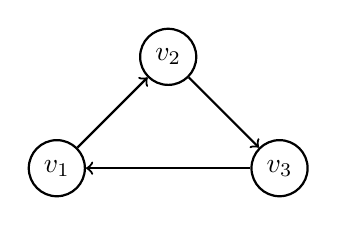
\begin{tikzpicture}[node distance={20mm}, thick, main/.style = {draw, circle}]
		\node[main] (2) {$v_{2}$};
		\node[main] (1) [below left of=2] {$v_{1}$};
		\node[main] (3) [below right of=2] {$v_{3}$};
		\path[->] (1) edge (2)
				  (2) edge (3)
				  (3) edge (1);
	\end{tikzpicture}
	\caption{Example for a polynomial for a graph $\overrightarrow{G}$.}
	\label{pol-ex}
\end{figure}

Now if we take $V(G) = \{v_{1}, \dots, v_{n}\}$ which map each one of them $v_{i} \to x_{i}$. Then for a assignment $\overrightarrow{c}$ as for each $i$ $v_i \to c_i$ we know that $G$ has a proper coloring iff $P_{\overrightarrow{G}}(\overrightarrow{c}) \neq 0$. That is if $S_{1}, \dots, S_{n}$ are lists of allowed colors for $v_{1}, \dots, v_{n}$ then $G$ is colorable from $S_{1}, \dots, S_{n}$ iff $(\exists c_{1} \in S_{1}, \dots, c_{n} \in S_{n}) P_{\overrightarrow{G}}(c_{1}, \dots, c_{n}) \neq 0$. To prove this we could use some theorem, but we will need a stronger version.

\begin{thm}[Combinatorial Nullstellensatz 2nd version]
	Let $f$ be a polynomial in $x_{1}, \dots, x_{n}$ and $S_{1}, \dots, S_{n} \subseteq \R$. If $(\exists d_{1}, \dots, d_{n})$ total degree $(f) \leq d_{1} + \dots + d_{n}$ and $[x_{1}^{d_{1}}\dots x_{n}^{d_{n}}]f \neq 0$ and $(\forall i) |S_{i}| > d_{i}$. Then $\exists c_{1} \in S_{1}, \dots, c_{n} \in S_{n} : f(c_{1}, \dots, c_{n}) \neq 0$.
\end{thm}

But why does it hold? We can assume $|S_{i}| = d_{i} + 1$. For the values $S_{i} = \{a_{1}, \dots, a_{d_{i}+1}\}$ (as colors). We know that if $x_{i} \in S$ then $(x_{i} - a_{1}) (x_{i} - a_{2}) \cdots (x_{i} - a_{d_{i}+1}) = 0$. Then $x_{i}^{d+1} - (a_{1} + \dots + a_{d+1}) x_{i}^{d_{i}} + \dots$ where we denote $b_{d_{i}} = (a_{1} + \dots + a_{d+1})$ so that leads to:

$$
x_{i}^{d_{i}+1} = b_{d_{i}}x_{i}^{d_{i}} + \dots + b_{1}x_{1} + b_{0}
$$

Now we may take a polynomial $f$ from the 2nd theorem. The polynomial $f'$ has the same values on $S_{1}, \dots, S_{n}$ but $\deg_{v_{i}}(f') \leq d_{i}$. So now the condition $(\forall i) |S_{i}| > \deg_{v_{i}} (f')$ holds. Only think is to see that $f' \not\equiv 0$.

We have already shown this theorem.

\begin{thm}
	If $[x_{1}^{d_1} \dots x_{n}^{d_n}]P \neq 0$, $d_1 + \dots + d_n = $ total degree of $P$, $S_1, \dots, S_{n}, (\forall i) |S_i| > d_i$ then $\Rightarrow (\exists c_{1} \in S_{1}, \dots, c_{n} \in S_{n}) P(c_{1}, \dots c_n) \neq 0$.
\end{thm}

\begin{observ}
	$P_{\overrightarrow{G}} (c_1, \dots, c_n) \neq 0 \Leftrightarrow c_1, \dots, c_n$ is a proper coloring of $G$.
\end{observ}

By combining these two results we may get a following corollary.

\begin{cor}
	If $[x_{1}^{d_1} \dots x_{n}^{d_n}]P_{\overrightarrow{G}} \neq 0$ and $L$ is a list assignment such that $(\forall i) |L(v_i)| > d$ then $G$ is $L$-colorable.
\end{cor}

\TODO{Complete this section.}